\documentclass{standalone}
\usepackage[svgnames]{xcolor}
\usepackage{tikz}
\usepackage{pgfplots}
\usetikzlibrary{arrows.meta,plotmarks,backgrounds}
\usepgfplotslibrary{fillbetween}
\tikzset{inner frame sep = 0pt, background rectangle/.style = { thick, draw = DarkBlue, fill = white }}
\pgfplotsset{
	compat = 1.18,
	layers/standard/.define layer set = {
		background,
		axis background,
		axis grid,
		axis ticks,
		axis lines,
		axis tick labels,
		pre main,
		main,
		axis descriptions,
		axis foreground
	}{
		grid style = { /pgfplots/on layer = axis grid },
		tick style = { /pgfplots/on layer = axis ticks },
		axis line style = { /pgfplots/on layer = axis lines },
		label style = { /pgfplots/on layer = axis descriptions },
		legend style = { /pgfplots/on layer = axis descriptions },
		title style = { /pgfplots/on layer = axis descriptions },
		colorbar style = { /pgfplots/on layer = axis descriptions },
		ticklabel style = { /pgfplots/on layer = axis tick labels },
		axis background@ style = { /pgfplots/on layer = axis background },
		3d box foreground style = { /pgfplots/on layer = axis foreground }
	},
    layers/axis on top/.define layer set = {
        background,
        axis background,
        pre main,
        main,
        axis grid,
        axis ticks,
        axis lines,
        axis tick labels,
        axis descriptions,
        axis foreground
    }{ /pgfplots/layers/standard }
}
\begin{document}
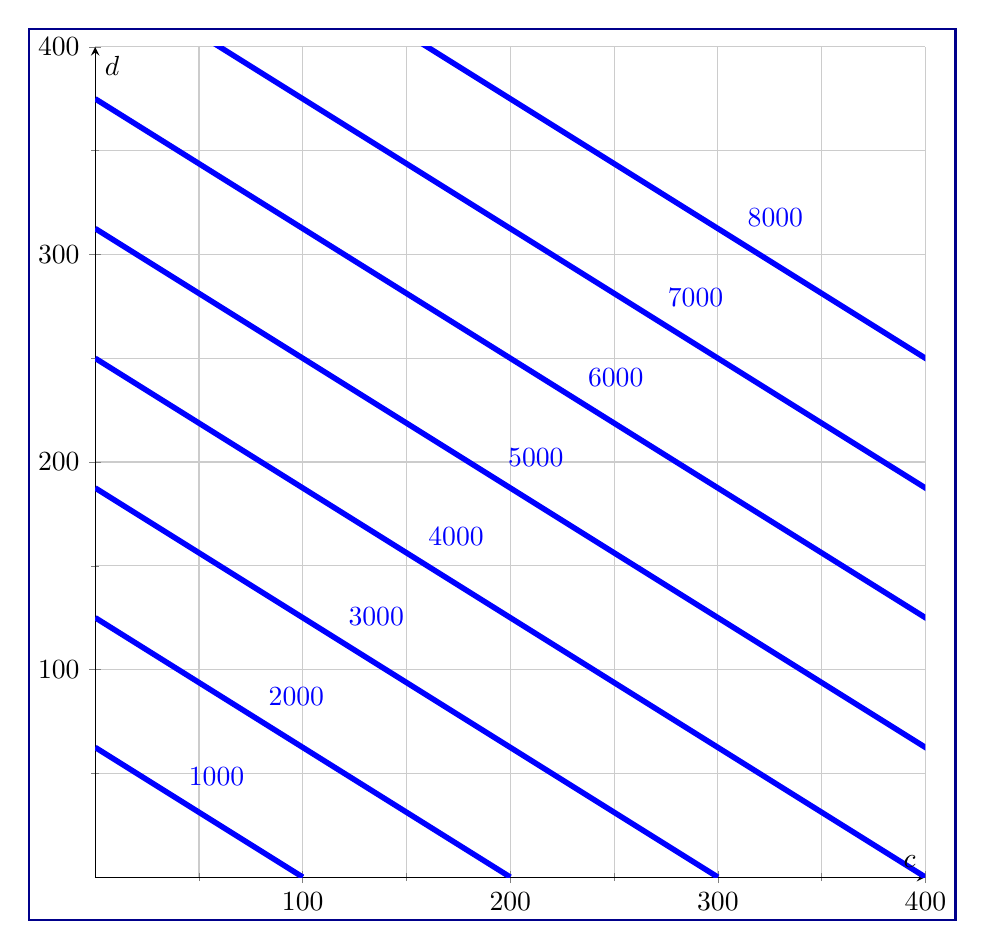
\begin{tikzpicture}[framed]
\begin{axis}
[
	trig format plots=rad,
	view={0}{90},
	scale only axis,
	height=300,
	width=300,
	axis x line=middle,
	axis y line=center,
	xlabel={\(c\)},
	ylabel={\(d\)},
	xtick distance=100,
	ytick distance=100,
	xmajorgrids=true,
	xminorgrids=true,
	minor x tick num=1,
	ymajorgrids=true,
	yminorgrids=true,
	minor y tick num=1,
	grid style={gray!40},
	xmin=0,
	xmax=400,
	ymin=0,
	ymax=400,
]
\definecolor{gray}{RGB}{128,128,128}
\path[name path=xaxis] (0, 0) -- (400,0);
\definecolor{blue}{RGB}{0,0,255}
\addplot[smooth, color=blue, line width=2pt, solid, domain=0:100, samples=30] {((1000-10*x)/16)};
\addplot[smooth, color=blue, line width=2pt, solid, domain=0:200, samples=30] {((2000-10*x)/16)};
\addplot[smooth, color=blue, line width=2pt, solid, domain=0:300, samples=30] {((3000-10*x)/16)};
\addplot[smooth, color=blue, line width=2pt, solid, domain=0:400, samples=30] {((4000-10*x)/16)};
\addplot[smooth, color=blue, line width=2pt, solid, domain=0:500, samples=30] {((5000-10*x)/16)};
\addplot[smooth, color=blue, line width=2pt, solid, domain=0:600, samples=30] {((6000-10*x)/16)};
\addplot[smooth, color=blue, line width=2pt, solid, domain=0:700, samples=30] {((7000-10*x)/16)};
\addplot[smooth, color=blue, line width=2pt, solid, domain=0:800, samples=30] {((8000-10*x)/16)};
\node[blue] at (axis cs: 58.4615384615385,48.4615384615385) {1000};
\node[blue] at (axis cs: 96.9230769230769,86.9230769230769) {2000};
\node[blue] at (axis cs: 135.384615384615,125.384615384615) {3000};
\node[blue] at (axis cs: 173.846153846154,163.846153846154) {4000};
\node[blue] at (axis cs: 212.307692307692,202.307692307692) {5000};
\node[blue] at (axis cs: 250.769230769231,240.769230769231) {6000};
\node[blue] at (axis cs: 289.230769230769,279.230769230769) {7000};
\node[blue] at (axis cs: 327.692307692308,317.692307692308) {8000};
\end{axis}
\end{tikzpicture}
\end{document}
